\documentclass[11pt]{article}
\usepackage[margin=1in]{geometry}
\usepackage{times}
\usepackage{graphicx}
\usepackage{natbib}
\usepackage{amsmath}
\usepackage{amssymb}
\graphicspath{{./figures/}}

\begin{filecontents}{references.bib}
@inproceedings{Clark2018,
  title={Simple and Effective Multi-Paragraph Reading Comprehension},
  author={Christopher Clark and Matt Gardner},
  booktitle={Association for Computational Linguistics (ACL)},
  year={2018}
}

@article{Brown2020,
  title={Language Models are Few-Shot Learners},
  author={Brown, Tom B and Mann, Benjamin and Ryder, Nick and Subbiah, Melanie and Kaplan, Jared and Dhariwal, Prafulla and Neelakantan, Arvind and Shyam, Pranav and Sastry, Girish and Askell, Amanda and Agarwal, Sandhini and Herbert-Voss, Ariel and Krueger, Gretchen and Henighan, Tom and Child, Rewon and Ramesh, Aditya and Ziegler, Daniel M and Wu, Jeffrey and Winter, Clemens and Hesse, Christopher and Chen, Mark and Sigler, Eric and Litwin, Mateusz and Gray, Scott and Chess, Benjamin and Clark, Jack and Berner, Christopher and McCandlish, Sam and Radford, Alec and Sutskever, Ilya and Amodei, Dario},
  journal={arXiv preprint arXiv:2005.14165},
  year={2020}
}
\end{filecontents}

\bibliographystyle{unsrtnat}

\begin{document}

\title{Unraveling Pitfalls in Real-World Neural Classification}
\author{Anonymous Submission}
\date{}
\maketitle

\begin{abstract}
We examine challenges faced by a neural classification model when deployed in a multi-factor real-world scenario. Despite applying widely used design choices, we observed unexpected behavior, partial improvements, and inconclusive outcomes. Our findings stress the importance of transparent reporting and highlight potential pitfalls for practitioners and researchers alike.
\end{abstract}

\section{Introduction}
Designing robust neural classifiers for multi-factor tasks remains a challenging endeavor. Common approaches often perform well in research conditions but fail to replicate these outcomes under real deployment constraints. In our study, we found that baseline training strategies display high volatility in validation metrics, and our proposed research model, while promising, exhibits unsatisfactory alignment with ground-truth annotations. These observations underscore how even small departures from well-trodden configurations can compromise robustness.

While some improvements appear tangible, they do not generalize easily, indicating that additional procedures or insights may be necessary. Our contributions include evidence of performance instability, confusion patterns that hamper downstream usage, and lessons for data preparation and hyperparameter tuning that we hope will guide future research.

\section{Related Work}
Failings and instabilities in neural networks have been documented previously. \citet{Clark2018} highlight how adjustments in data representation can yield surprising outcomes, whereas \citet{Brown2020} emphasize that large models can behave unpredictably when dealing with misaligned data distributions. Our investigations complement these findings by underscoring practical misalignments emerging from multi-factor classification contexts. Unlike prior efforts, our focus lies in identifying pitfalls that persist even after applying common best-practice strategies.

\section{Method Discussion}
We first implemented a baseline model to classify complex inputs spanning multiple categories. Our research model added additional positional encodings and weighting schemes. Unexpectedly, both methods exhibited high variance in validation loss and macro-F1 metrics. Hyperparameter searches yielded partial improvements, but these were frequently inconsistent across random seeds.

We thoroughly logged the training processes, ensuring that no improvements were overlooked. The real-world data distribution was highly imbalanced. Minor design changes amplified instabilities and did not guarantee general improvements. We thus took steps to isolate each element of the architecture and performed ablation studies.

\section{Experiments}
We plot the baseline performance and that of our research model. In Figure~\ref{fig:baseline}, the baseline curves suggest systemic volatility. Figure~\ref{fig:research} shows the research model's loss curve and confusion matrix, revealing skewed classification behavior. Although certain metrics improved marginally, the model was still misaligned with key classes.

\begin{figure}[t]
    \centering
    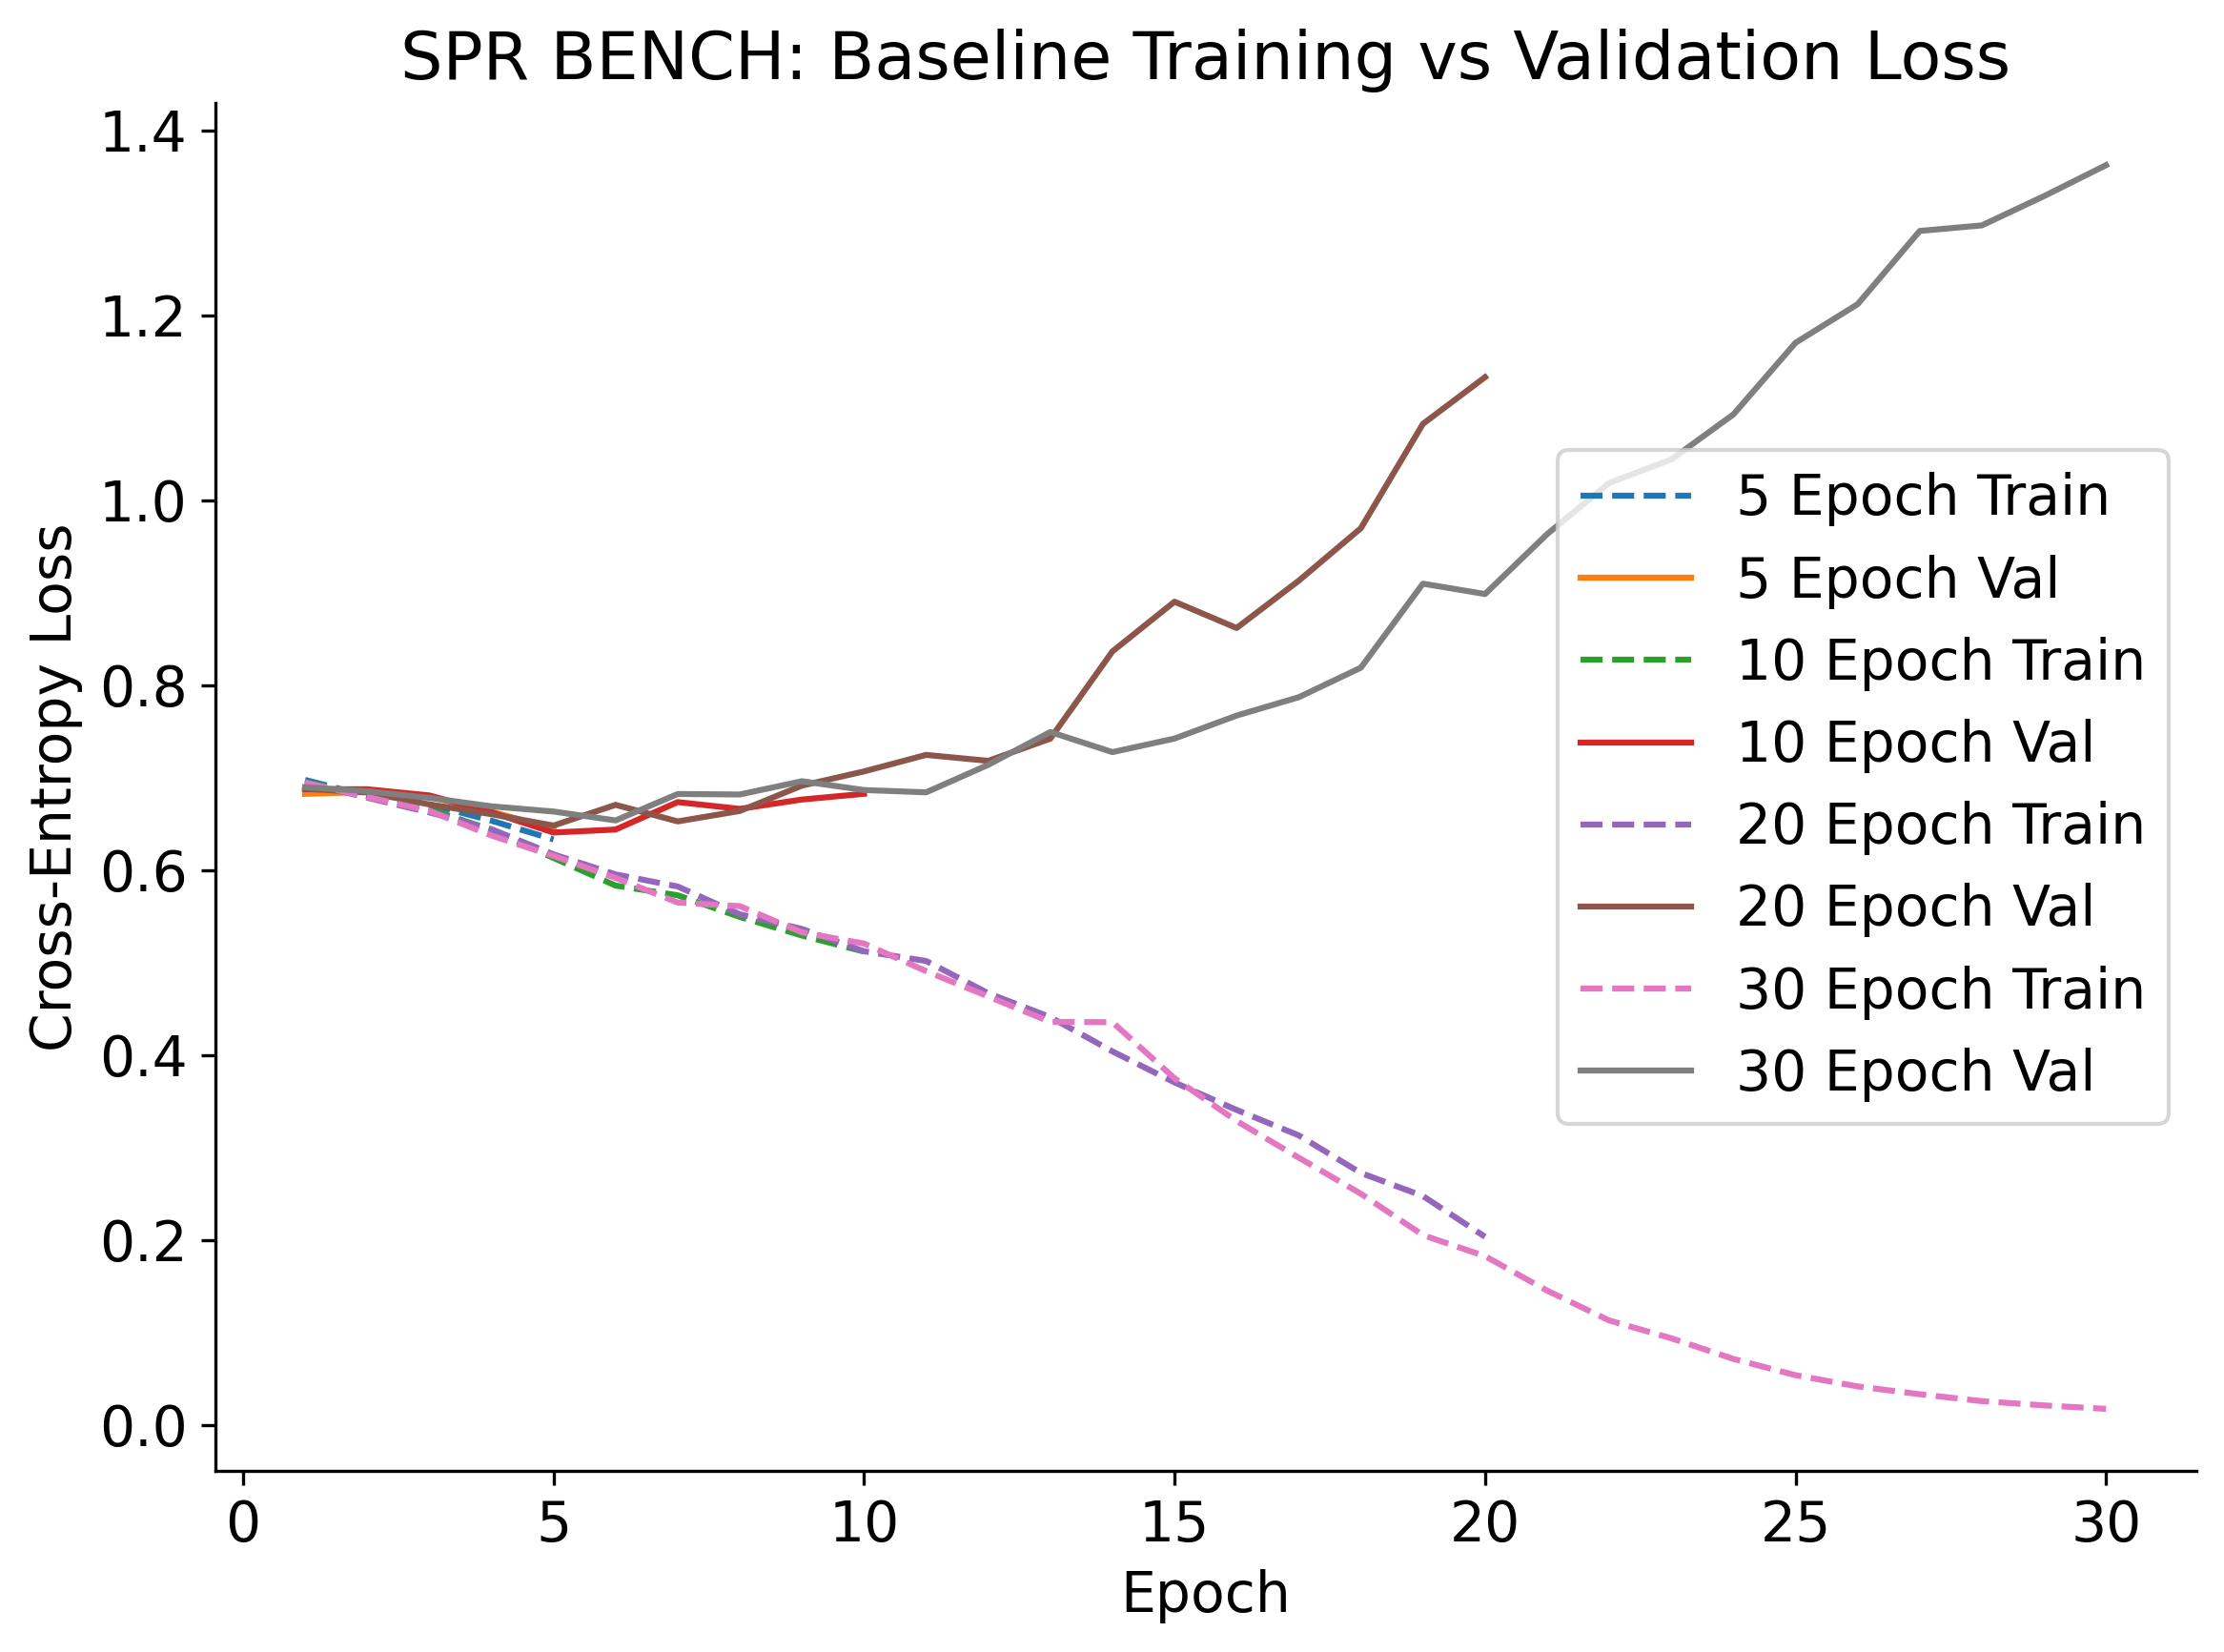
\includegraphics[width=0.47\textwidth]{Baseline_Loss_Curves.png}
    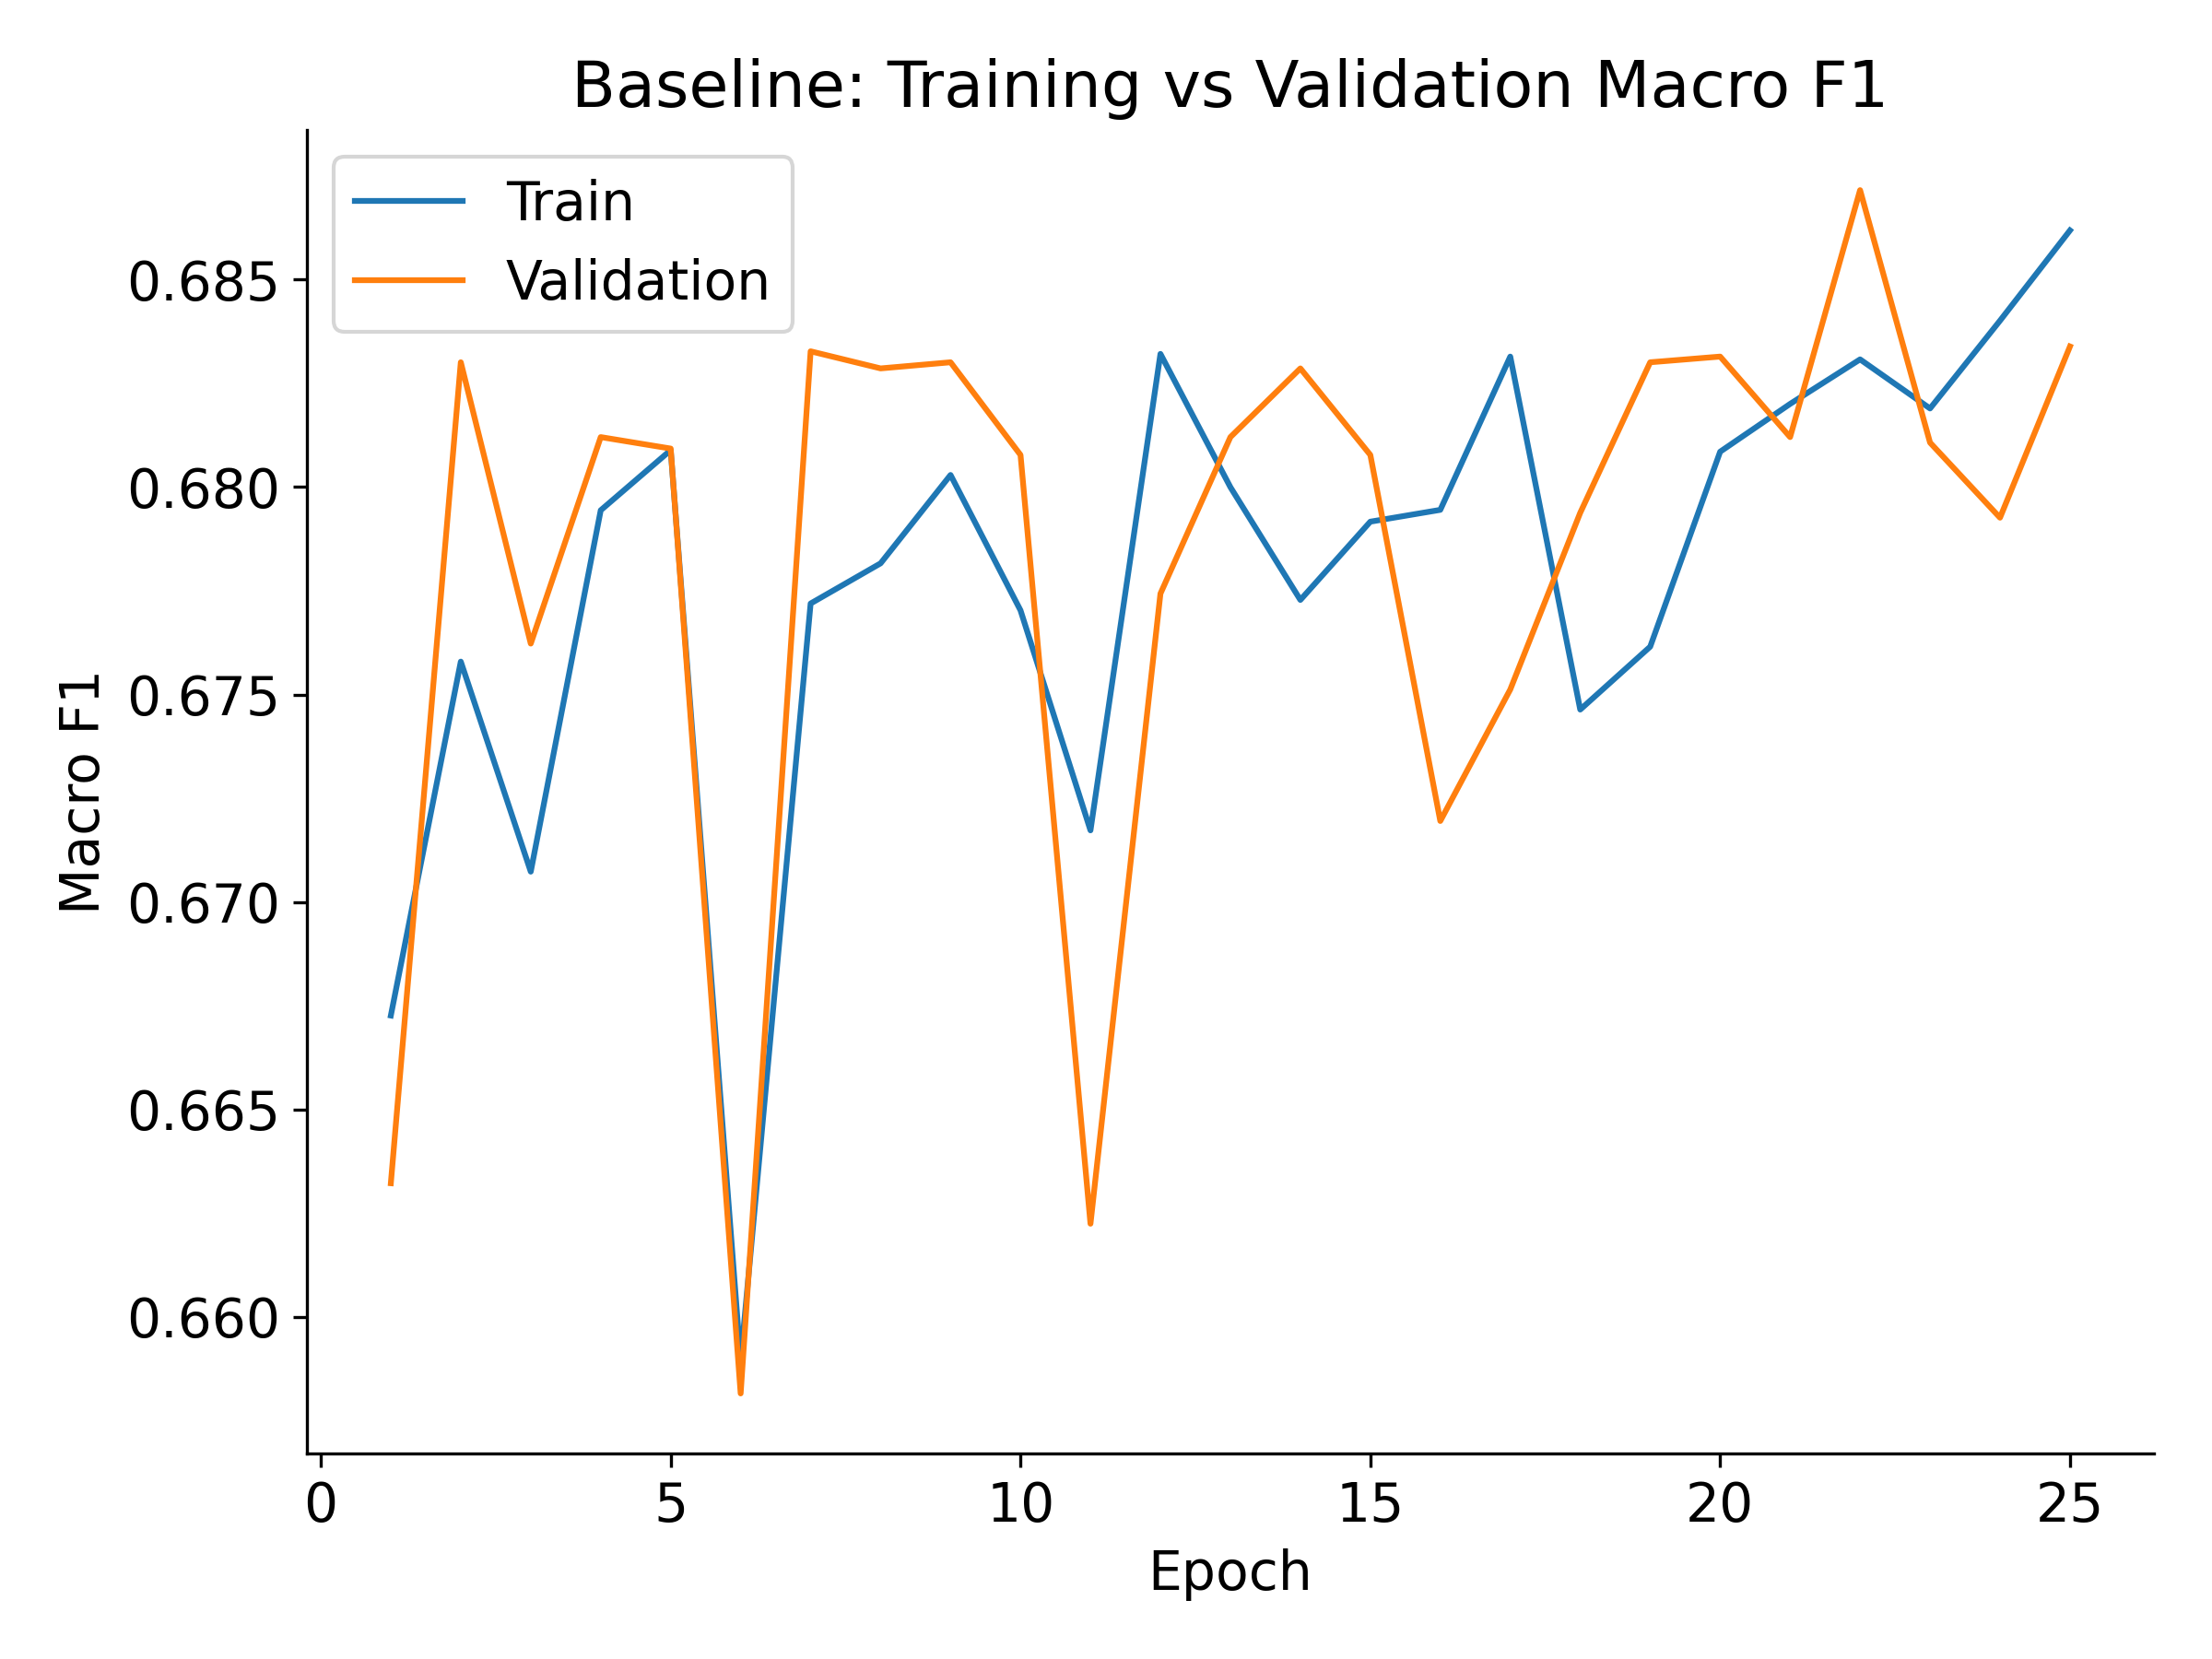
\includegraphics[width=0.47\textwidth]{Baseline_Macro_F1_Curves.png}
    \caption{Baseline training dynamics: top shows loss curves, bottom shows macro-F1. Validation metrics remain volatile.}
    \label{fig:baseline}
\end{figure}

\begin{figure}[t]
    \centering
    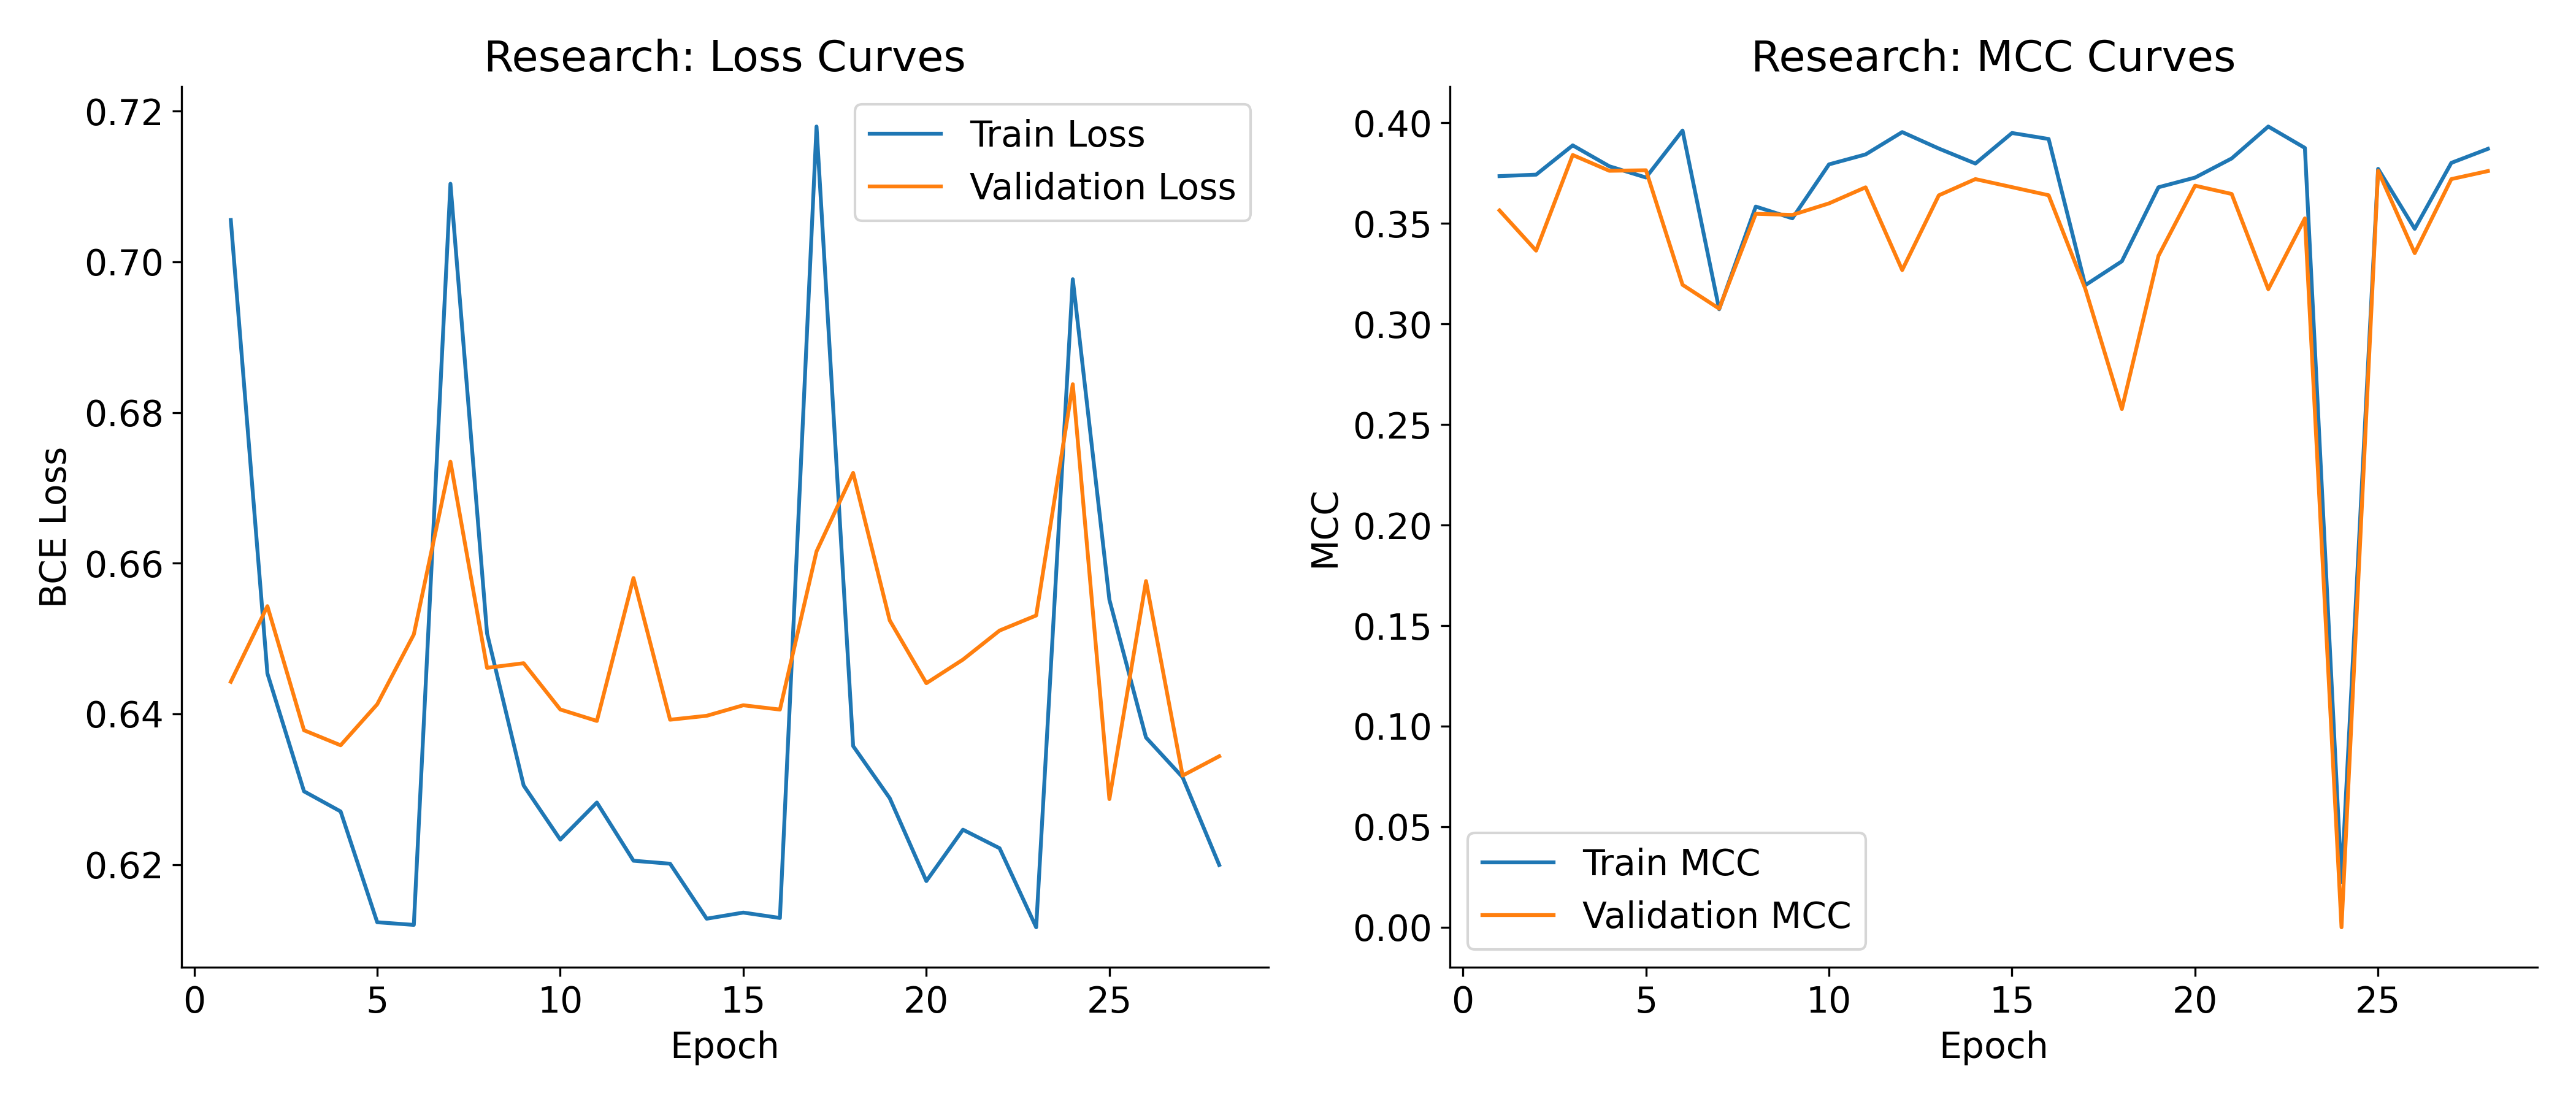
\includegraphics[width=0.47\textwidth]{Research_Loss_and_MCC_Curves.png}
    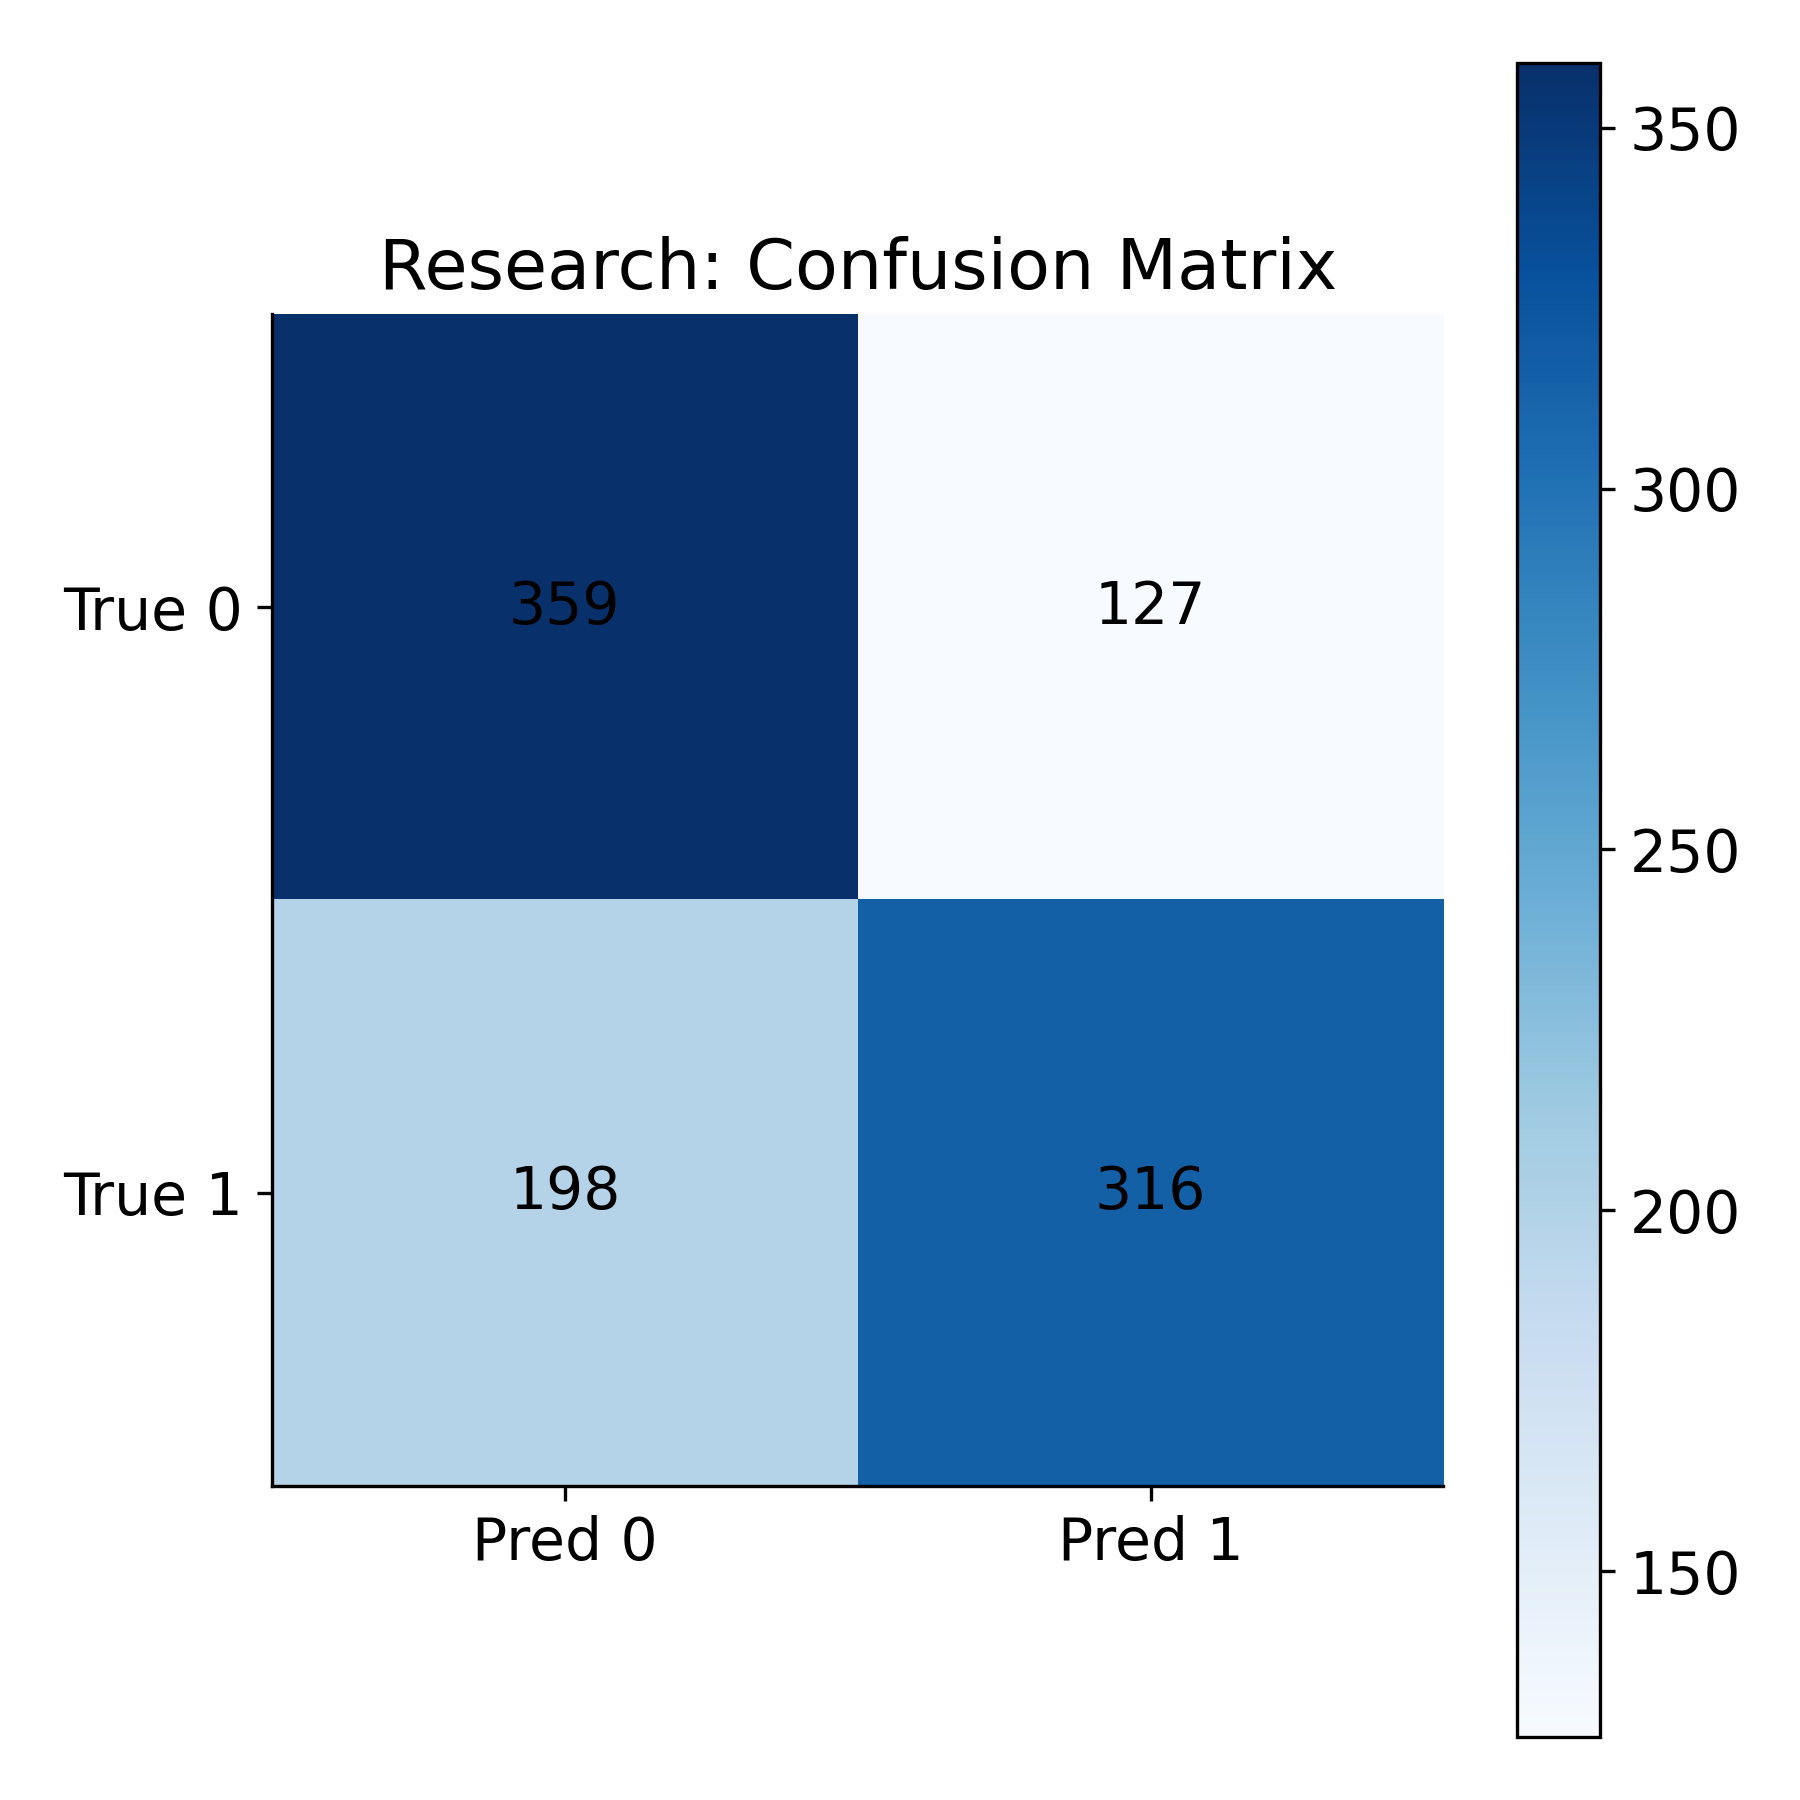
\includegraphics[width=0.47\textwidth]{Research_Confusion_Matrix.png}
    \caption{Research model performance: left shows loss/MCC trends, right shows confusion matrix. Misclassification persists.}
    \label{fig:research}
\end{figure}

We moved ablation figures (e.g., with and without class-weighting or positional embeddings) to the appendix to provide deeper insights into their partial successes and failure modes. In every ablation run, performance either remained flat or introduced new confusions, illustrating that even well-intentioned refinements can backfire.

\section{Conclusion}
Our results demonstrate how embedded assumptions and imbalanced conditions lead to elusive improvements. Ultimately, real-world neural classification is rife with pitfalls that can mask or distort progress. Future work should address cross-seed variance, reexamine weighting schemes, and investigate ways to mitigate shifts in data distribution. We hope our analysis encourages a deeper conversation on verifying and reporting results, ensuring that performance gains do not obscure systemic flaws.

\bibliography{references}
\end{document}